\chapter{Mockups}
\label{chapter:Mockups}
The tool used for this project to design the initial idea of the website was \textbf{Figma}, which allows us to design an interface that, according to our beliefs, aligns with the needs and expectations of the users.

Figma is a powerful tool for prototyping and interface design, enabling the creation of interactive and collaborative layouts in real time.

Below are some images of the mockup created, and the following link leads to the Figma project for a more detailed analysis if desired.

\textbf{SPLASH:}

\url{https://www.figma.com/design/73s1I8BXApUguw381t41PD/SPLASH?node-id=9-87&t=9a5nUxewcWEebZo4-1}

\begin{figure}[H]
      \centering
      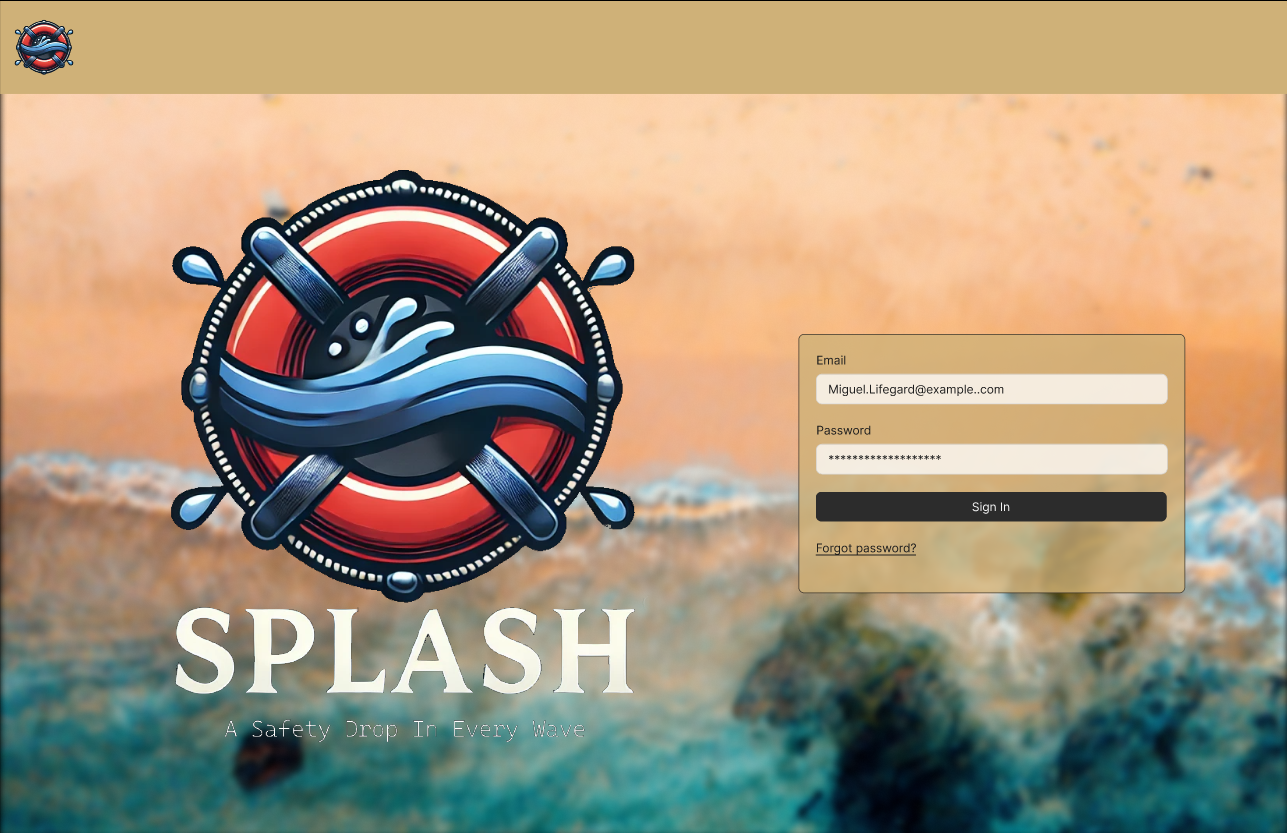
\includegraphics[width=13cm,height=7cm]{figs/Mockups/Login.png}
      \caption{SPLASH: Login page}
      \label{fig:Login}
\end{figure}

\begin{figure}[H]
      \centering
      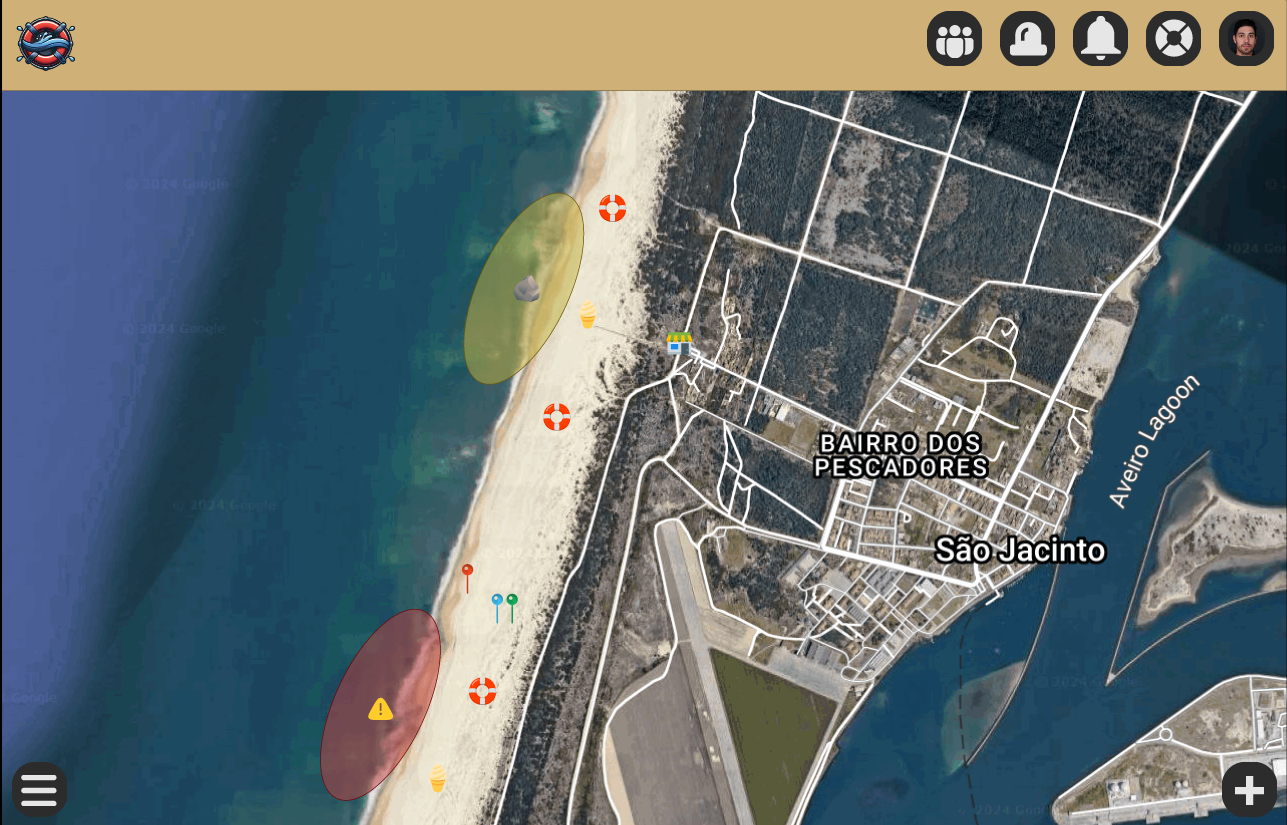
\includegraphics[width=13cm,height=7cm]{figs/Mockups/MAP.png}
      \caption{SPLASH: Interactive map page}
      \label{fig:Login}
\end{figure}

\begin{figure}[H]
      \centering
      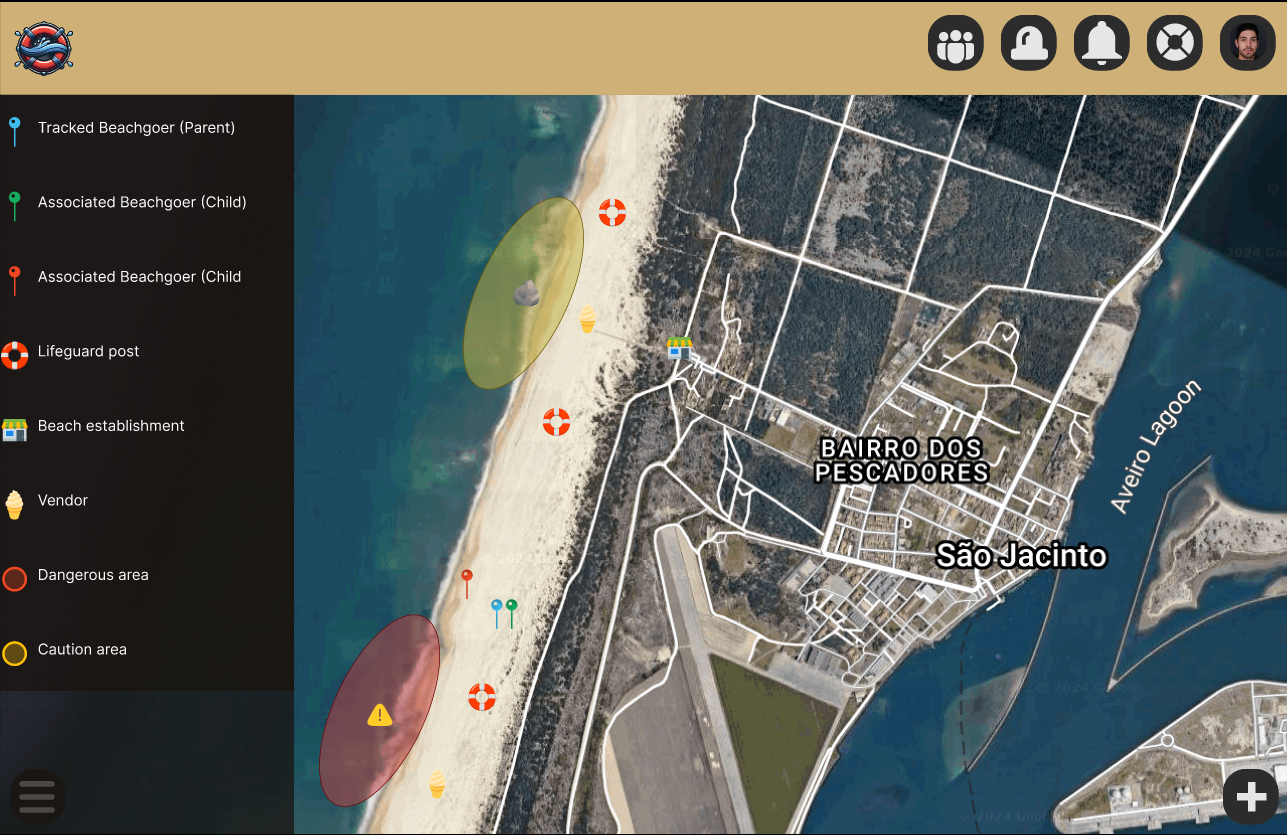
\includegraphics[width=13cm,height=7cm]{figs/Mockups/MAP_index.png}
      \caption{SPLASH: Index menu open in map}
      \label{fig:Login}
\end{figure}

\begin{figure}[H]
      \centering
      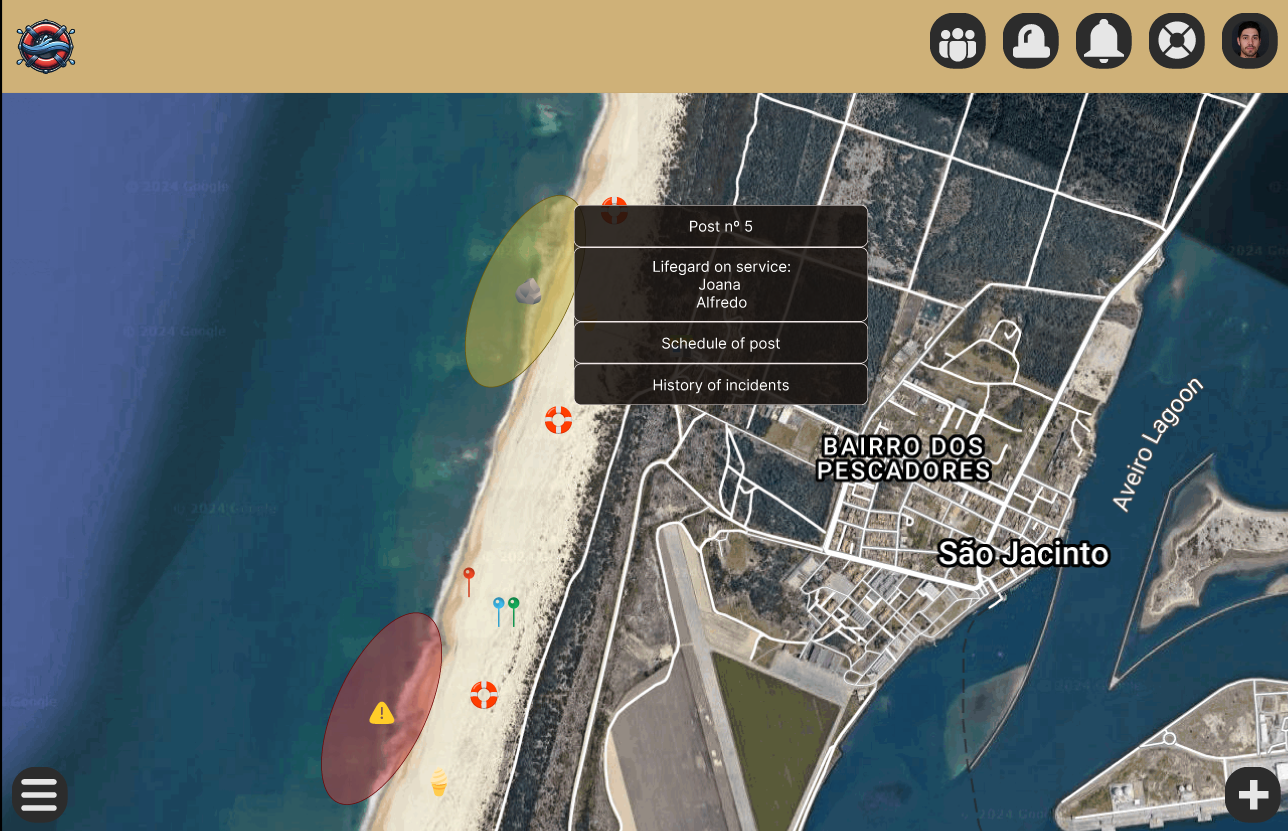
\includegraphics[width=13cm,height=7cm]{figs/Mockups/MAP_popup.png}
      \caption{SPLASH: Popup in map}
      \label{fig:Login}
\end{figure}

\begin{figure}[H]
      \centering
      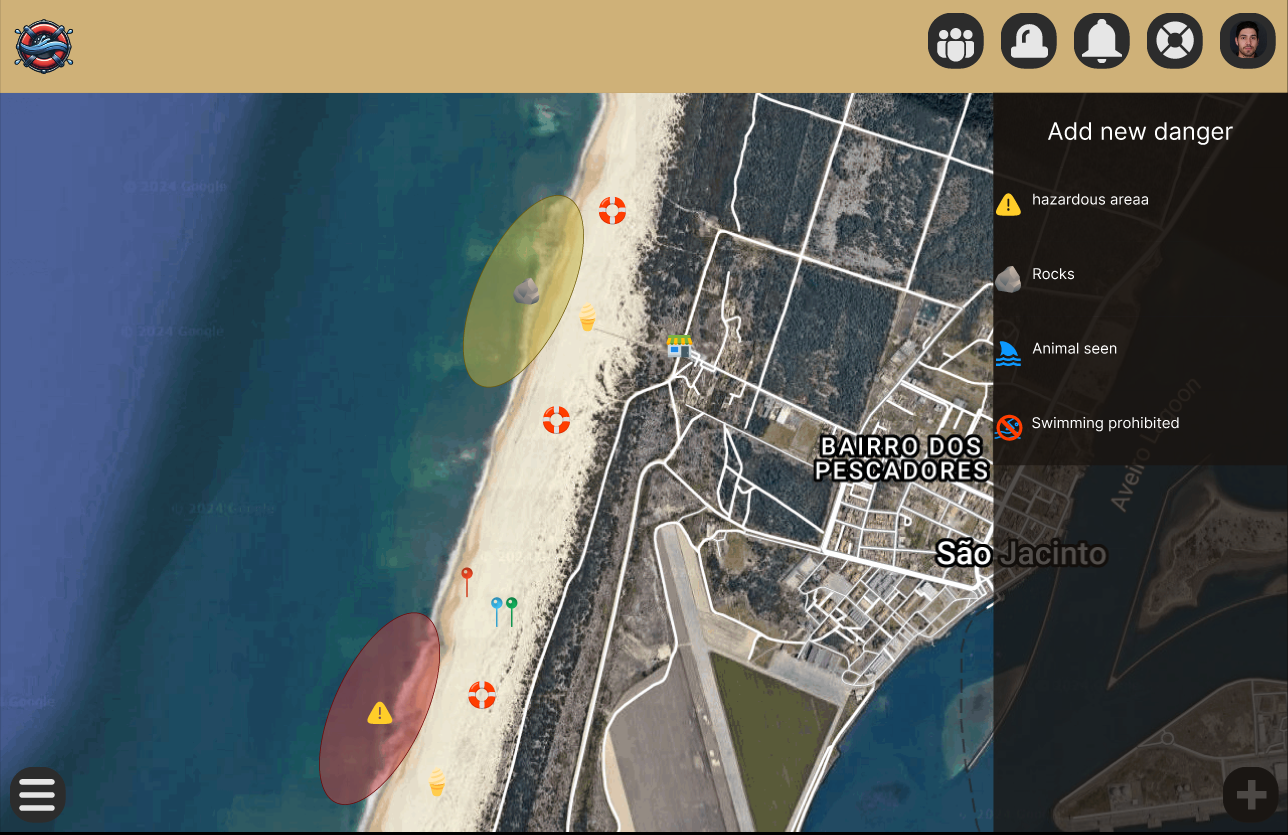
\includegraphics[width=13cm,height=7cm]{figs/Mockups/MAP_add1.png}
      \caption{SPLASH: Add hazard menu open in map}
      \label{fig:Login}
\end{figure}

\begin{figure}[H]
      \centering
      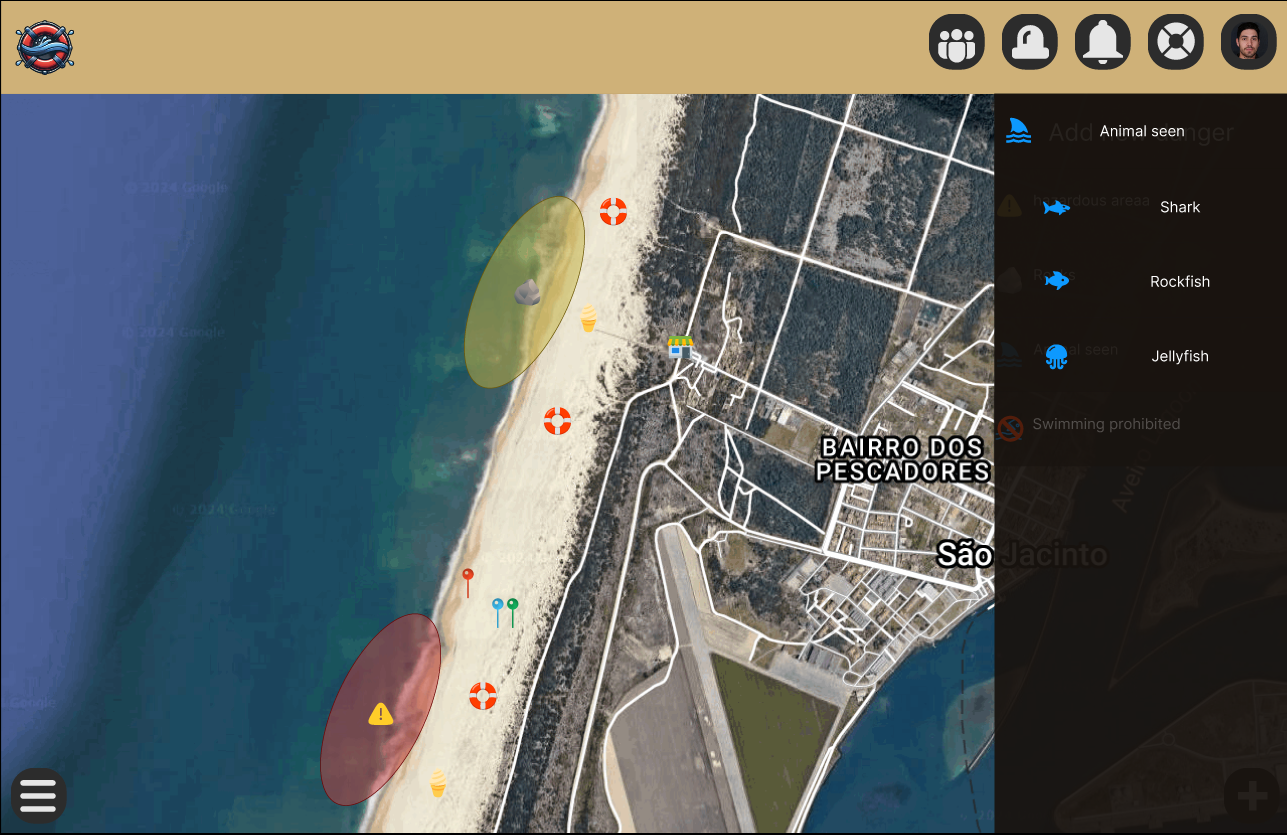
\includegraphics[width=13cm,height=7cm]{figs/Mockups/MAP_add2.png}
      \caption{SPLASH: Type of hazard menu open in map}
      \label{fig:Login}
\end{figure}